\scanpage{25}
1) gr. alg $\boxed{G}$ sur $\mathbf Q_p$.

2) hom continu
\[
\boxed{\rho:\pi\mathrel{\unsure{-|\longrightarrow}}G(\mathbf Q_p)}
\]
d'où
\diagram{\begin{tikzcd}[column sep=small,row sep=small]
& \unsure{Q|\Phi}_\Omega^! \arrow[dl,dash] \arrow[dr,dash] & \\
G_\Omega^! &&G_\Omega
\end{tikzcd}}

\margin{unique}
\margin{\deleted{\unsure{fg}}}
\figure{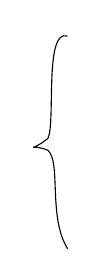
\begin{tikzpicture}[x=1cm,y=1cm]
\draw (0.3,2.7) .. controls (0,2.8) and (0.15,1.6) .. (0.05,1.4)
 .. controls (-0.2,1.2) and (-0.2,1.35) .. (0.05,1.25)
 .. controls (0.22,1.1) and (0.05,0.4) .. (0.3,0);
\end{tikzpicture}}
3)
\[
\boxed{G_{m\Omega}\xrightarrow{j^!}G_\Omega^!}
\]
d'où
\diagram{\begin{tikzcd}[column sep=small,row sep=large]
& Q_\Omega=\tau\wedge_{G_{m\Omega}}\unsure{Q|\Phi}_\Omega^! \arrow[dl,dash] \arrow[dr,dash] & \\
G''_\Omega=(\tau^{\unsure{*}}\wedge_{G_{m\Omega}}(G_\Omega^!,\mathrm{int})) && G_\Omega
\end{tikzcd}}
\[
\overbrace{j_\Omega:G_m\longrightarrow G''_\Omega}
\]

4) $\boxed{Q_L\text{ sur }G_L}$ descendant $Q_\Omega$ sur $G_\Omega$.
\diagram{\begin{tikzcd}[column sep=small]
U''_L\subset G''_L \arrow[r,dash] & Q_L \arrow[r,dash] & G_L
\end{tikzcd}}
\[
,\quad j_L:G_{mL}\mathrel{\unsure{-|\longrightarrow}}G''_L
\]

5) \deleted{Un \unsure{ensemble} $\boxed{\Delta}$ d'opérations
\inserted{\figure{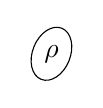
\begin{tikzpicture}[baseline=-.4ex]\draw[rotate=-22] (0,0) ellipse (.24 and .35);\node at (0,0) {$\rho$};\end{tikzpicture}}} de $\Gamma\ (\supset\pi)$ sur $Q_\Omega$
\margin{\unsure{commutant}}
\inserted{d'où $\Gamma\longrightarrow G''_L(\Omega)=G''_\Omega(\Omega)$}
\unsure{prolongeant} celle de $\pi$, \unsure{comp.} avec celle de $\Gamma$ sur $\Omega$

tel que si $\rho$ \unsure{est telle}, \unsure{par des} \unsure{formant} orbite sous $U''_L$
opérant par (pour $u\in U''_L(L)$)
\[
(u.\rho)(\gamma)=\tau u\{\rho(\gamma)\}\tau u^{-1}
=\unsure{(\mathrm{int}\,\tau(u)).\rho(\gamma)|(\mathrm{int}\,\tau(u).\rho)(\gamma)}
\]
i.e.
\[
\unsure{u-\rho|u.\rho}=\mathrm{int}\,\tau(u)\rho)
\]
[NB si $u\rho=\rho$ i.e. $\deleted{\unsure{\tau u.\rho}}\ \rho$ commutant à $\tau(u)$ pour
\margin{\unsure{donc|pour}}
}
\figure{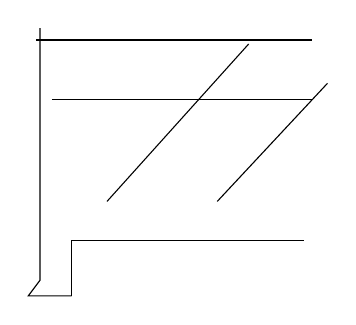
\begin{tikzpicture}[x=1cm,y=1cm]
\draw (0.15,3.4)--(0.15,0.2)--(0,0)--(0.55,0);
\draw (0.55,0)--(0.55,0.7)--(3.5,0.7);
\draw (0.1,3.25)--(3.6,3.25);
\draw (0.3,2.5)--(3.6,2.5);
\draw (1,1.2)--(2.8,3.2);
\draw (2.4,1.2)--(3.8,2.7);
\end{tikzpicture}}

Un torseur (\unsure{non nullité}) \inserted{à droite $\uline{\Delta}$}
$\unsure{R_0|P_0}$ sous $U''_L(L)$, et
un $U''_L(L)$-\uline{hom de}
\diagram{\begin{tikzcd}[column sep=large]
\rho:\Delta\arrow[r] &
\begin{array}{l}
\mathrm{Op.}\text{ de }\Gamma\text{ sur }(\Omega,Q_L,G_L)\\
\text{qui sont compatibles avec}\\
\text{\unsure{l'op. donnée|l'op. qui}}\text{ de }\Gamma\text{ sur }\Omega,\\
\text{et celle de }\pi\unsure{\in|\subset}\Gamma\text{ sur }Q_L\ldots
\end{array}
\end{tikzcd}}
\figure{\begin{tikzpicture}[x=1cm,y=1cm]
\draw (0.1,1.6)..controls (0,1.5) and (0,0.2)..(0,0)--(2.3,0);
\end{tikzpicture}}
lorsque on fait opérer $U''_L(L)$ \inserted{à droite} sur le deuxième ens. par
\[
u.\alpha=\tau(\alpha)u\tau(\alpha)^{-1}
\]
\margin{24}
